\documentclass[aspectratio=169]{beamer}
\usepackage[utf8]{inputenc}
\usepackage{graphics}
\usepackage{booktabs} %za tabelu

\usetheme[sectionstyle=style2]{trigon}
\titlegraphic{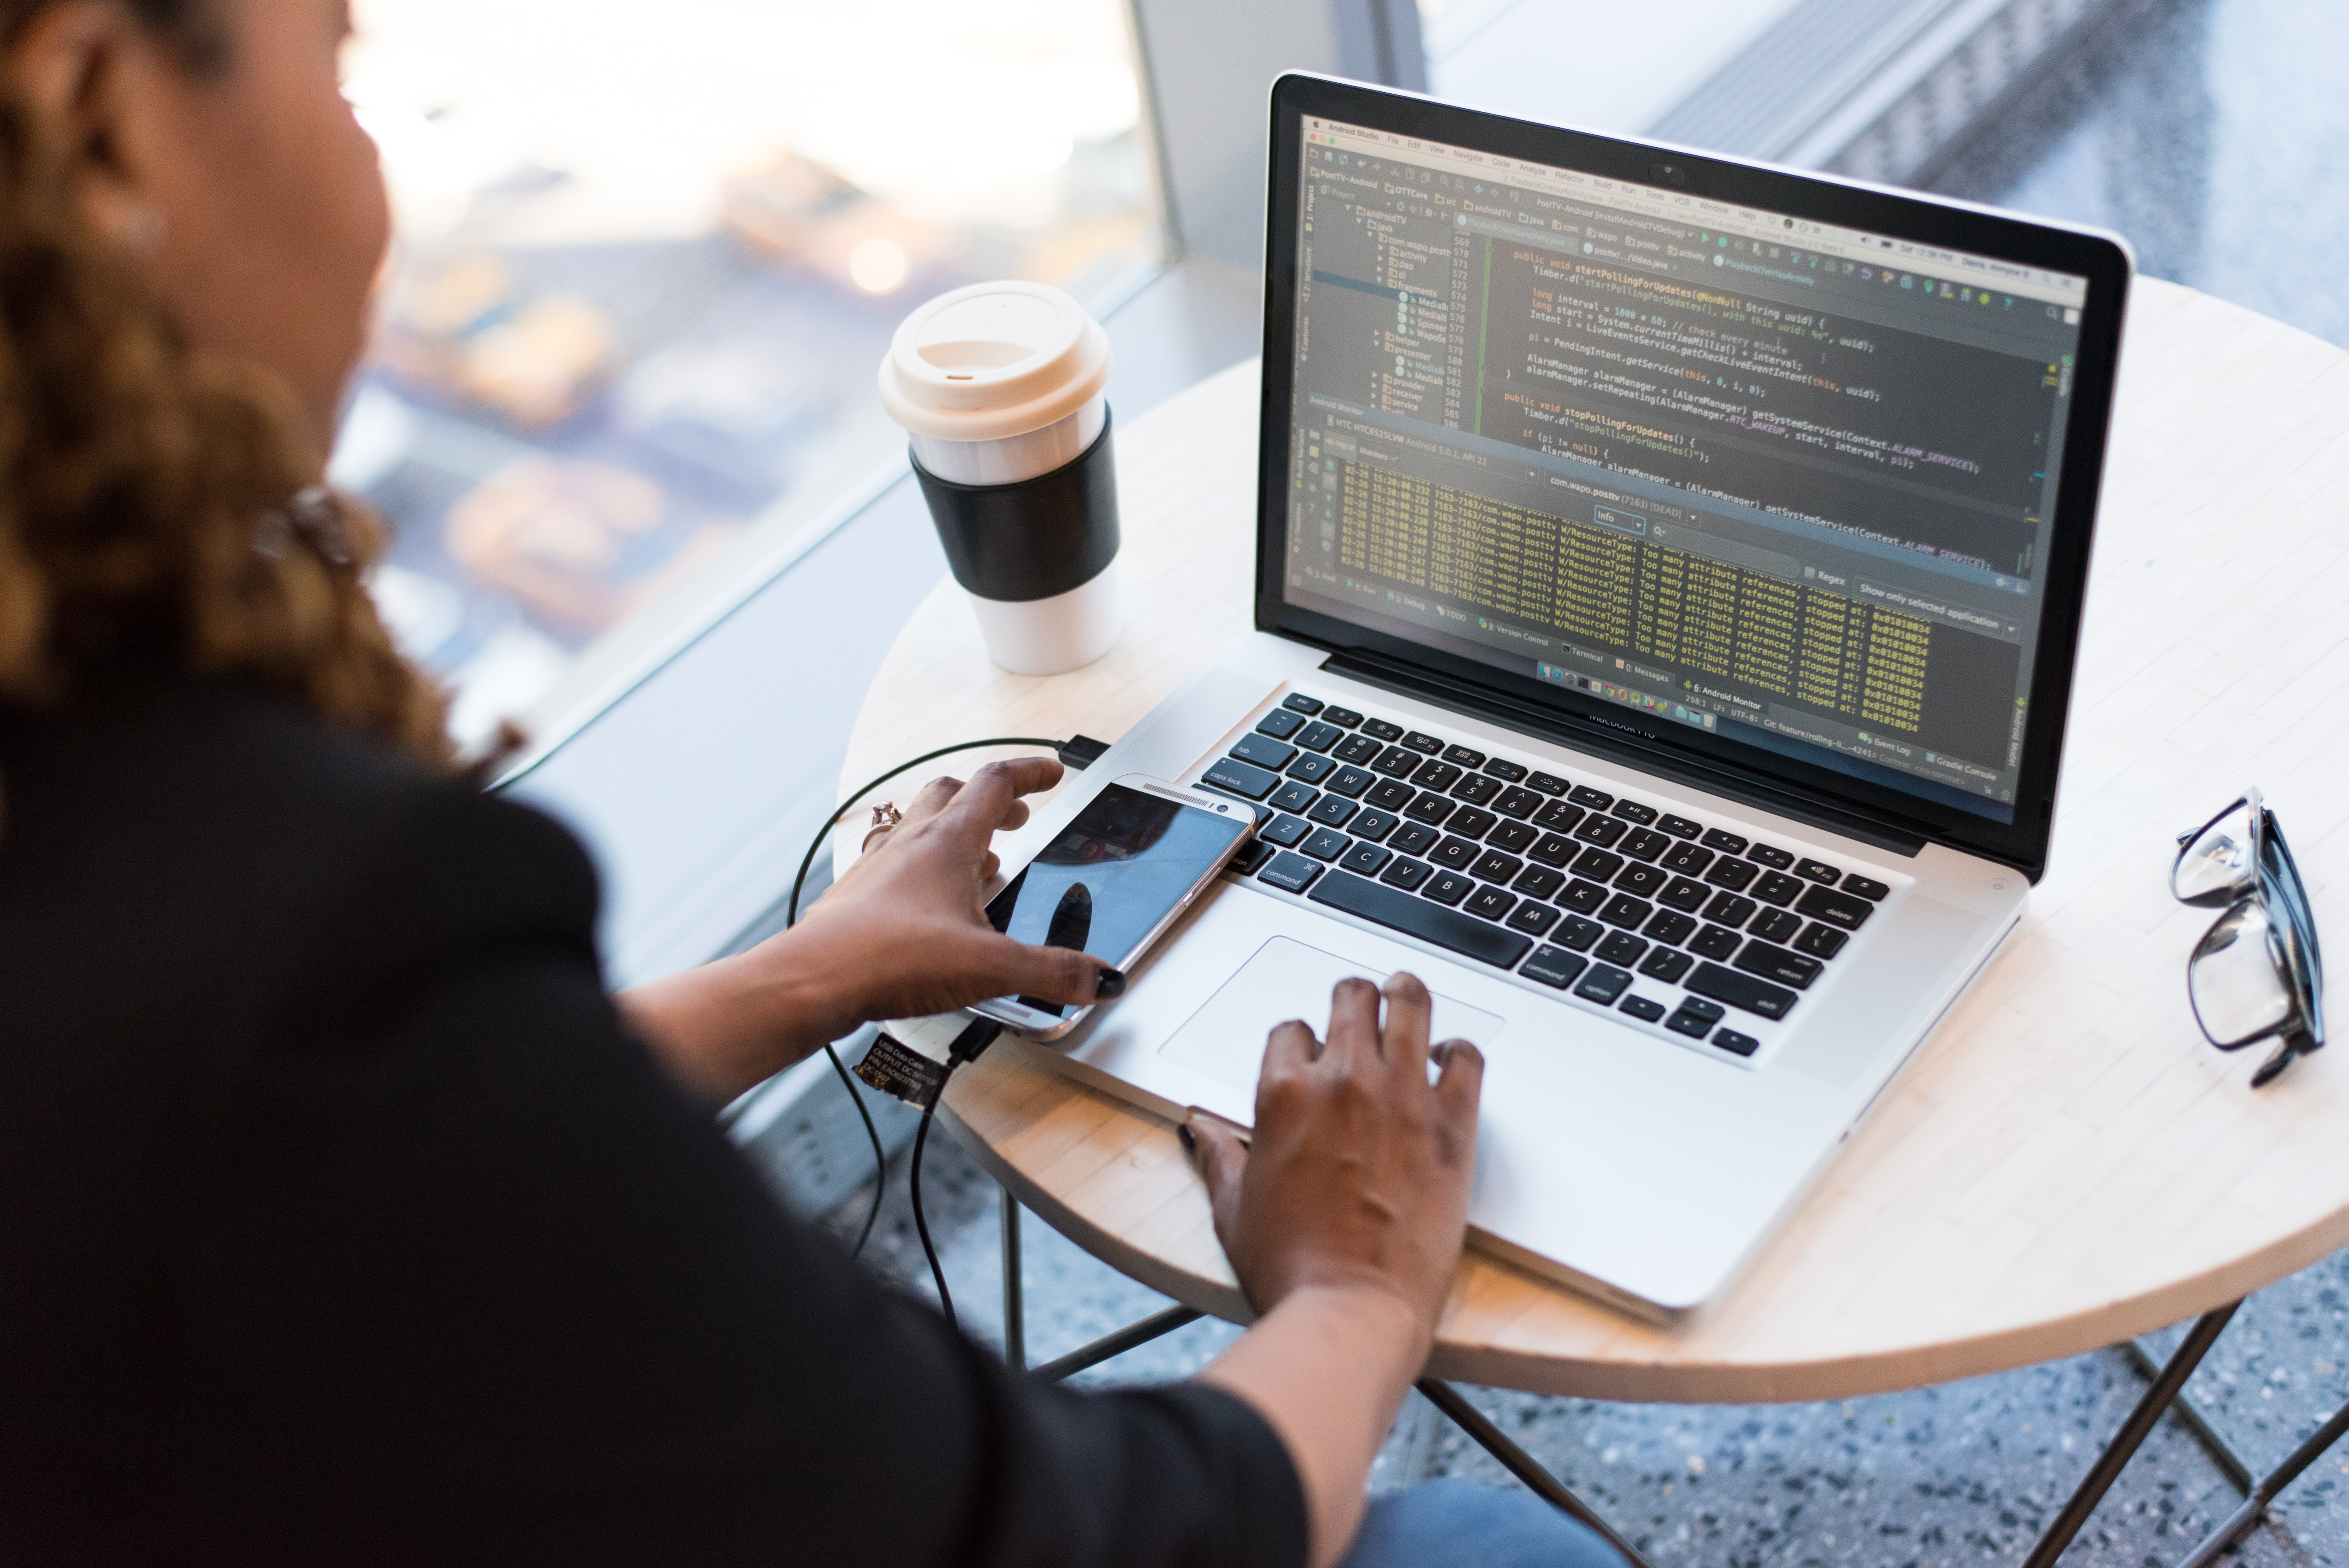
\includegraphics[height=\paperheight]{slika1.jpg}} %slika na prvom slajdu
\biglogo{LOGO-1.png} %logo na pocetnom slajdu

\title{Žene u računarstvu}
\author{ Zorana Jevtić \and Bojana Zagorac\\  \and Miloš Bigović  \and Jelena Veličković\\}
\date{Decembar 2022}



%==============================================================================
%                               BEGIN DOCUMENT
%==============================================================================


\begin{document}

\titleframe  %za pravljenje pocetnog slajda
\setbeamertemplate{frame footer}{Zorana Jevtic, Bojana Zagorac, Milos Bigovic, Jelena Velickovic}

%==============================================

\begin{frame}{Sadržaj}
  \setbeamertemplate{section in toc}[sections numbered]
  \tableofcontents[hideallsubsections]
\end{frame}

%==============================================
\section{Ada Bajron}
%==============================================



%==============================================
\section{Margaret Hamilton}
%==============================================



%==============================================
\section{Eniac programeri}
%==============================================



%==============================================
\section{Zastupljenost žena u IT sektoru}
%==============================================

\begin{frame}{Statistika}

    \begin{itemize}
        \item<1-> Posle Drugog svetskog rata, programiranje je postalo popularnije medju oba pola.
        
        \item<2->Do sredine ‘80-ih godina procenat zena na kompjuterskim naukama rastao je veoma brzo
        
        \item<3-> Kada su zene pocele da u ovoj oblasti cine vise od \alert{37\%} studenata, procenat je poceo naglo da pada sve do danas 
    \end{itemize}

    \begin{table}[h]
        \centering
        \begin{tabular}{c|c}
        \toprule
                Godina    & procenat zena u IT-u \\ 
        \midrule
                1984       & 37\%  \\ 
                1990-2010  & 18\%  \\ 
                2019       & 13\%  \\ 
        \bottomrule
        \end{tabular}
    \end{table}

\end{frame}

%------------------------------------------------

{\usebackgroundtemplate{
\includegraphics[width=\paperwidth, height=\paperheight]{slika8.jpg}}
\begin{frame}
  
    \begin{columns}
        \column{0.5\textwidth}
        \begin{block}{Zasto tako malo zena ulazi u IT}
            \begin{itemize}
            \item<1-> Zene su manje zainteresovane?
            \item<2-> Kultura, stetni stereotipi
            \item<3-> nedostatak podrske na skolskom nivou 
            \item<4-> nedostatak zenskih uzora
            \end{itemize}
        \end{block}  

        \column{0.5\textwidth}
        \begin{block}{Buducnost zena u IT-u}
            \begin{itemize}
                \item<5-> Industrija kompjuterskih nauka raste izuzetnom brzinom

                \item<6-> Da bi se ovaj problem rešio potrebno je da se žene u IT-u više promovišu

                \item<7-> Twitter, Instagram, TikTok su uveli razne heštegove kojim podržavaju i podstiču rad žena u IT kompanijama 
            \end{itemize}
        \end{block}        
    \end{columns}
   
\end{frame}
}

%=================================================

{\usebackgroundtemplate{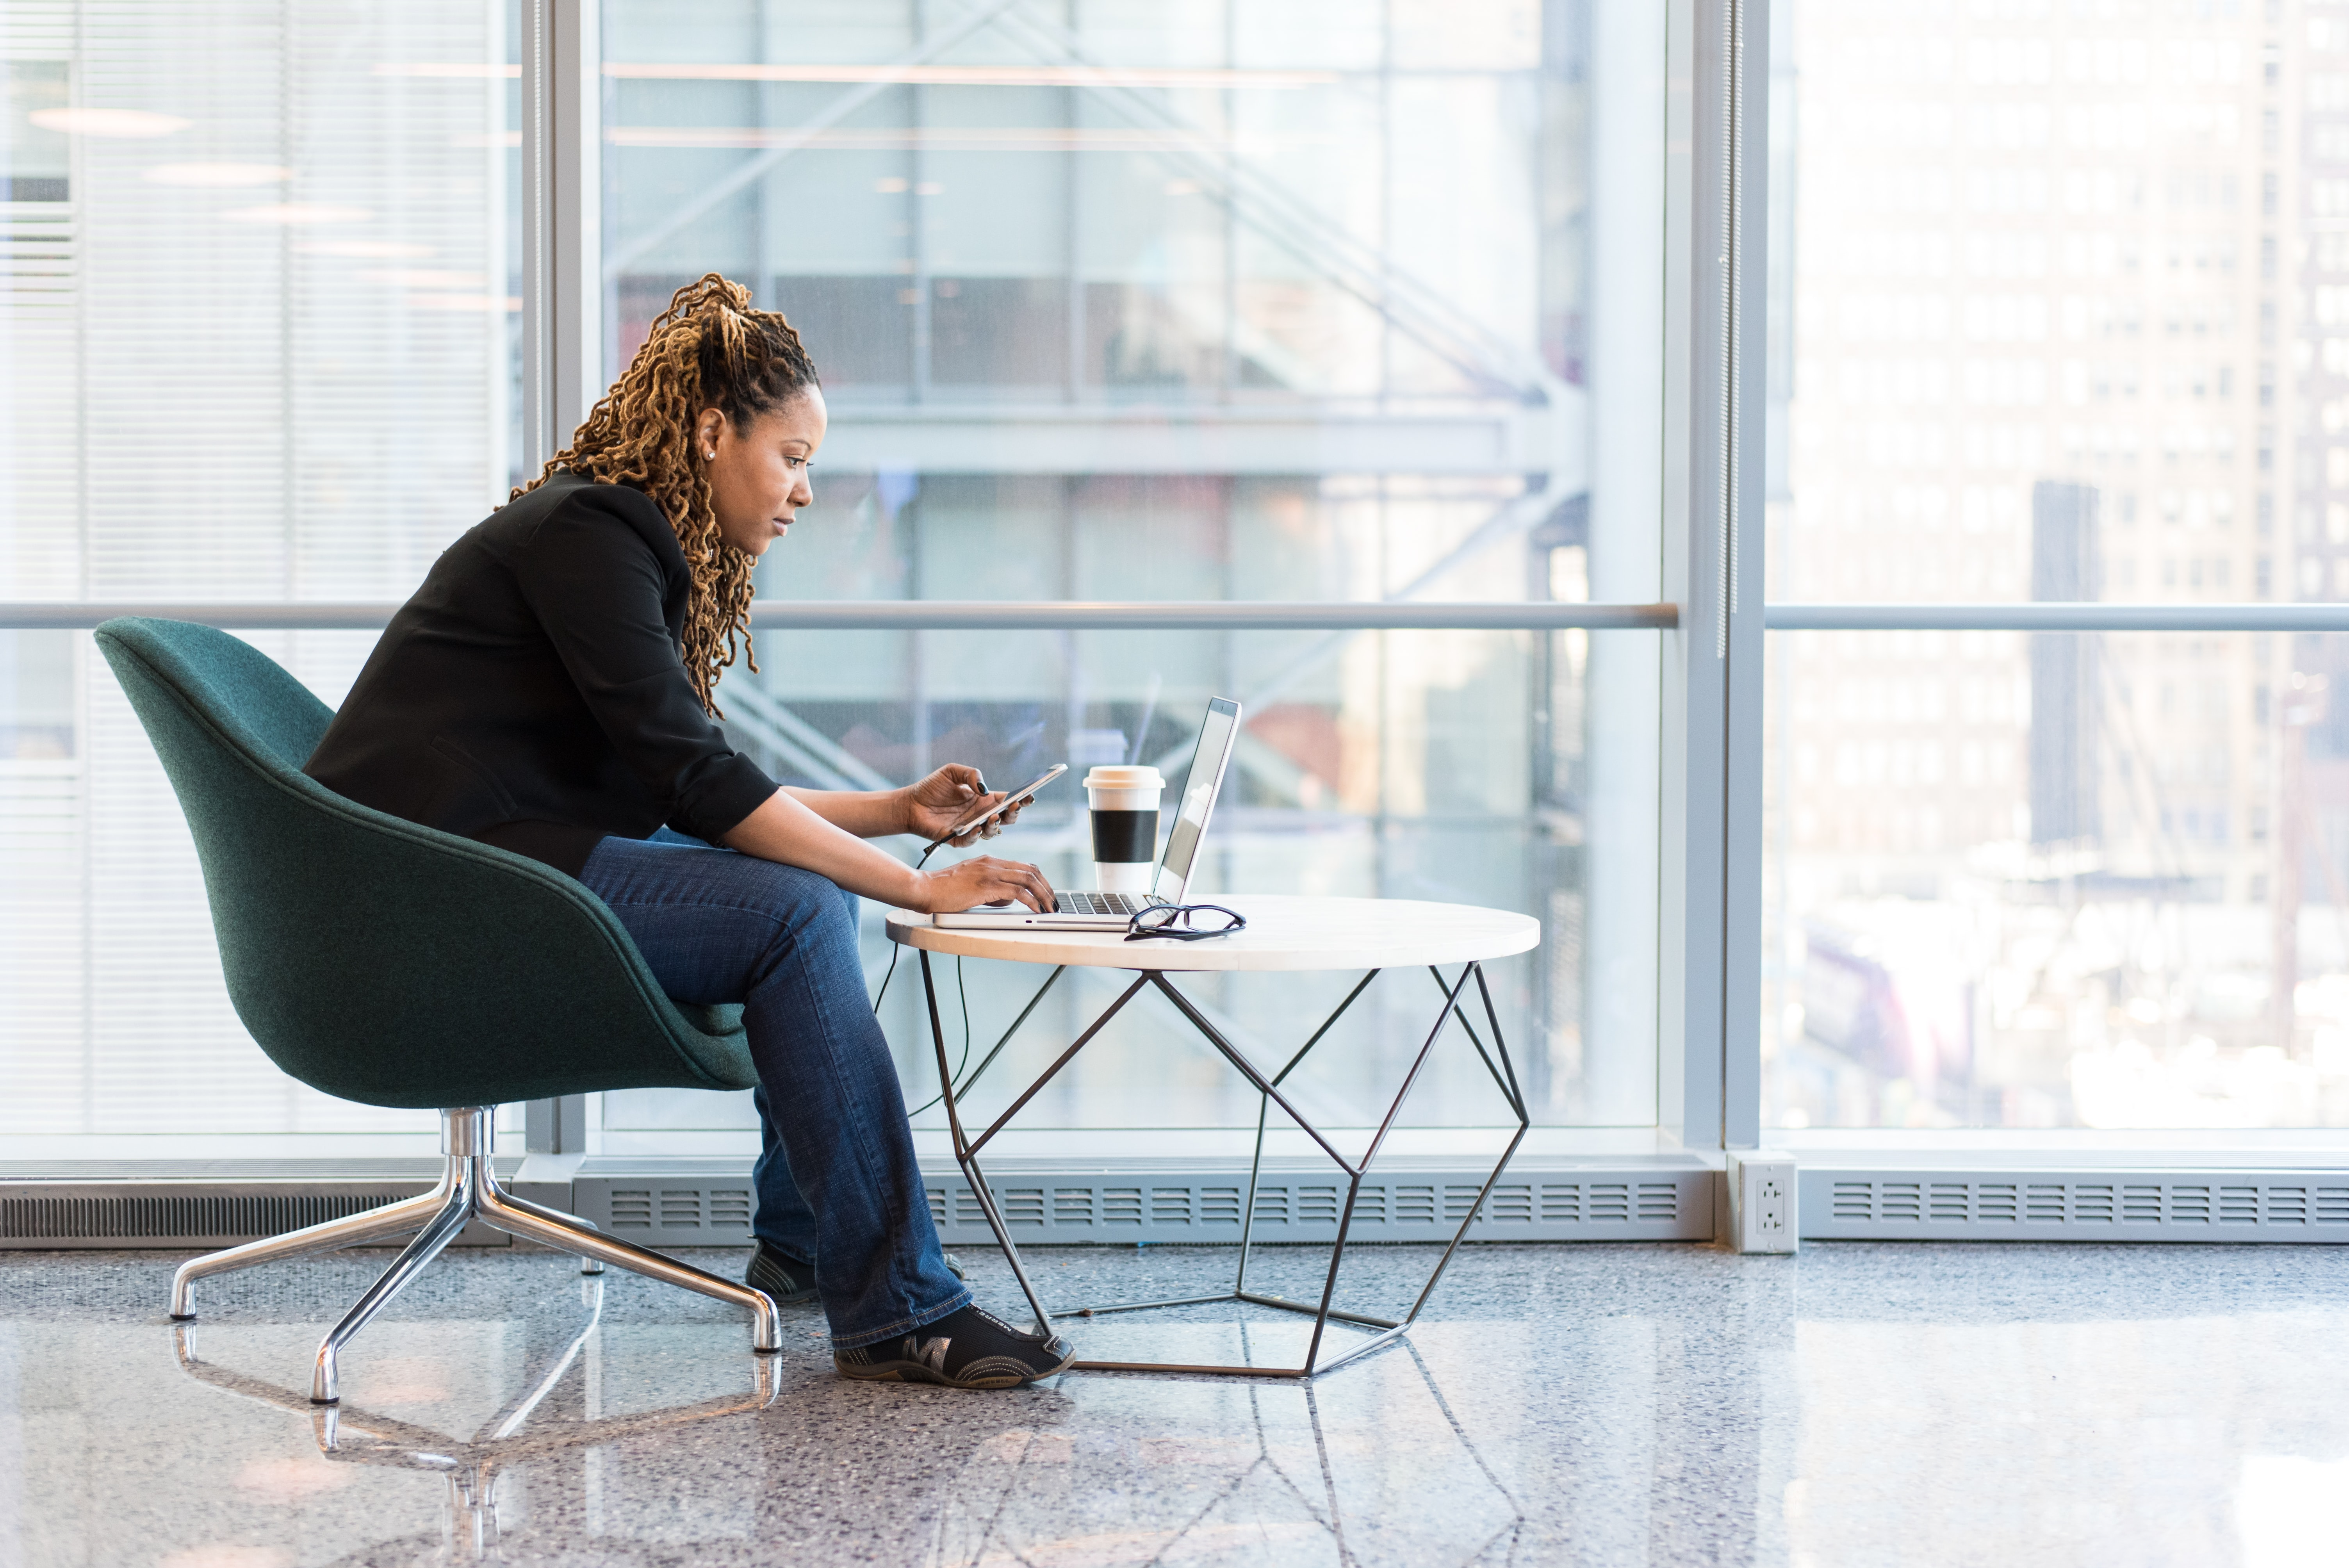
\includegraphics[width=\paperwidth, height=\paperheight]{slika2.jpg}}
\begin{frame}
    \centering
   \textbf{\Huge{KRAJ}} 
\end{frame}
}

\end{document}
